
%%--------------------------------------------------
%% Halliday: Fundamentals of Physics
%%--------------------------------------------------


%% Chapter 11: Rolling, Torque, and Angular Momentum
%%--------------------------------------------------


%% Learning Objectives
%%--------------------------------------------------

%% 11.01: Identify that smooth rolling can be considered as a combination of pure translation and pure rotation.
%% 11.02: Apply the relationship between the center-of-mass speed and the angular speed of a body in smooth rolling.


%% Halliday Multiple Choice Questions
%%--------------------------------------------------
\element{halliday-mc}{
\begin{question}{halliday-ch11-q01}
    A wheel rolls without sliding along a horizontal road as shown. 
    %% NOTE: is this sentence really necessary?
    %The velocity of the center of the wheel is represented by $\longrightarrow$. 
    \begin{center}
    \begin{tikzpicture}
        %% Ground
        \node[anchor=north,fill,pattern=north east lines,minimum width=6cm, minimum height=0.1cm] at (0,0) {};
        \draw (-3,0) -- (3,0);
        %% Wheel
        \draw[thick] (0,1.5) circle (1.5);
        \draw[thick,->] (0,1.5) ++ (135:1) arc (135:45:1);
        \draw[fill] (0,0) circle (1.5pt) node[pos=1.0,anchor=south] {$P$};
        \draw[thick,->] (2,1.5) -- ++(0:1) node[pos=0.5,anchor=south] {$\vec{v}$};
    \end{tikzpicture}
    \end{center}
    Point $P$ is painted on the rim of the wheel. 
    The instantaneous velocity of point $P$ is:
    \begin{multicols}{3}
    \begin{choices}
        \AMCboxDimensions{down=-0.4cm}
        \wrongchoice{
            \begin{tikzpicture}
                \draw[white] (0,0) rectangle (1,1);
                \draw[fill] (0,0.5) circle (1.5pt);
                \draw[very thick,->] (0,0.5) -- ++(0:1);
            \end{tikzpicture}
        }
        \wrongchoice{
            \begin{tikzpicture}
                \draw[white] (0,0) rectangle (1,1);
                \draw[fill] (1,0.5) circle (1.5pt);
                \draw[very thick,->] (1,0.5) -- ++(180:1);
            \end{tikzpicture}
        }
        \wrongchoice{
            \begin{tikzpicture}
                \draw[white] (0,0) rectangle (1,1);
                \draw (0.5,0) circle (1.5pt);
                \draw[very thick,->] (0.5,0) -- ++(90:1);
            \end{tikzpicture}
        }
        \wrongchoice{
            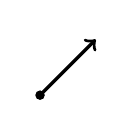
\begin{tikzpicture}
                \draw[white] (0,0) rectangle (1,1);
                \draw[fill] (0.15,0.15) circle (1.5pt);
                \draw[very thick,->] (0.15,0.15) -- ++(45:1);
            \end{tikzpicture}
        }
        %% ANS is E
        \correctchoice{
            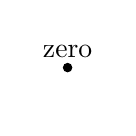
\begin{tikzpicture}
                \draw[white] (0,0) rectangle (1,1);
                \draw[fill] (0.5,0.5) circle (1.5pt) node[anchor=south] {zero};
            \end{tikzpicture}
        }
    \end{choices}
    \end{multicols}
\end{question}
}

\element{halliday-mc}{
\begin{question}{halliday-ch11-q02}
    A wheel of radius \SI{0.5}{\meter} rolls without sliding on a horizontal surface as shown. 
    Starting from rest,
        the wheel moves with constant angular acceleration \SI{6}{\radian\per\second\squared}.
    \begin{center}
    \begin{tikzpicture}
        %% Ground
        \node[anchor=north,fill,pattern=north east lines,minimum width=6cm, minimum height=0.1cm] at (0,0) {};
        \draw (-3,0) -- (3,0);
        %% Wheel
        \draw[thick] (0,1.5) circle (1.5);
        \draw[thick,->] (0,1.5) ++ (135:1) arc (135:45:1);
        \draw[fill] (0,1.5) circle (1.5pt);
        \draw[thick,->] (2,1.5) -- ++(0:1) node[pos=0.5,anchor=south] {$\vec{v}$};
    \end{tikzpicture}
    \end{center}
    The distance traveled by the center of the wheel from $t=0$ to $t=\SI{3}{\second}$ is:
    \begin{multicols}{2}
    \begin{choices}
        \wrongchoice{zero}
        \wrongchoice{\SI{27}{\meter}}
      \correctchoice{\SI{13.5}{\meter}}
        \wrongchoice{\SI{18}{\meter}}
        \wrongchoice{none of the provided}
    \end{choices}
    \end{multicols}
\end{question}
}

\element{halliday-mc}{
\begin{question}{halliday-ch11-q03}
    Two wheels roll side-by-side without sliding, at the same speed. 
    The radius of wheel 2 is twice the radius of wheel 1. 
    The angular velocity of wheel 2 is:
    \begin{choices}
        \wrongchoice{twice the angular velocity of wheel 1}
        \wrongchoice{the same as the angular velocity of wheel 1}
      \correctchoice{half the angular velocity of wheel 1}
        \wrongchoice{more than twice the angular velocity of wheel 1}
        \wrongchoice{less than half the angular velocity of wheel 1}
    \end{choices}
\end{question}
}

\element{halliday-mc}{
\begin{question}{halliday-ch11-q04}
    A forward force on the axle accelerates a rolling wheel on a horizontal surface. 
    If the wheel does not slide the frictional force of the surface on the wheel is:
    \begin{choices}
        \wrongchoice{zero}
        \wrongchoice{in the forward direction}
        \wrongchoice{in the backward direction}
      \correctchoice{in the upward direction}
        \wrongchoice{in the downward direction}
    \end{choices}
\end{question}
}

\element{halliday-mc}{
\begin{question}{halliday-ch11-q05}
    When the speed of a rear-drive car is increasing on a horizontal road
        the direction of the frictional force on the tires is:
    \begin{choices}
        \wrongchoice{forward for all tires}
        \wrongchoice{backward for all tires}
        \wrongchoice{forward for the front tires and backward for the rear tires}
      \correctchoice{backward for the front tires and forward for the rear tires}
        \wrongchoice{zero}
    \end{choices}
\end{question}
}

\element{halliday-mc}{
\begin{question}{halliday-ch11-q06}
    A solid wheel with mass $M$, radius $R$, and rotational inertia $M R^2/2$,
        rolls without sliding on a horizontal surface. 
    A horizontal force $F$ is applied to the axle and the center of mass has an acceleration $a$. 
    The magnitudes of the applied force $F$ and the frictional force $f$ of the surface,
        respectively, are:
    \begin{multicols}{2}
    \begin{choices}
        \wrongchoice{$F = Ma$,\phantom{2} $f = \text{zero}$}
        \wrongchoice{$F = Ma$,\phantom{2} $f = \dfrac{M a}{2}$}
        \wrongchoice{$F = 2Ma$, $f = M a$}
        \wrongchoice{$F = 2Ma$, $f = \dfrac{M a}{2}$}
      \correctchoice{$F = \dfrac{3Ma}{2}$, $f = \dfrac{M a}{2}$}
    \end{choices}
    \end{multicols}
\end{question}
}

\element{halliday-mc}{
\begin{question}{halliday-ch11-q07}
    The coefficient of static friction between a certain cylinder and a horizontal floor is \num{0.40}. 
    If the rotational inertia of the cylinder about its symmetry axis is given by $I = \frac{1}{2} M R^2$,
        then the magnitude of the maximum acceleration the cylinder can have without sliding is:
    \begin{multicols}{3}
    \begin{choices}
        \wrongchoice{$0.1 g$}
        \wrongchoice{$0.2 g$}
        \wrongchoice{$0.4 g$}
      \correctchoice{$0.8 g$}
        \wrongchoice{$g$}
    \end{choices}
    \end{multicols}
\end{question}
}

\element{halliday-mc}{
\begin{question}{halliday-ch11-q08}
    A thin-walled hollow tube rolls without sliding along the floor. 
    The ratio of its translational kinetic energy to its
        rotational kinetic energy (about an axis through its center of mass) is:
    \begin{multicols}{3}
    \begin{choices}
      \correctchoice{\num{1}}
        \wrongchoice{\num{2}}
        \wrongchoice{\num{3}}
        \wrongchoice{\num{1/2}}
        \wrongchoice{\num{1/3}}
    \end{choices}
    \end{multicols}
\end{question}
}

\element{halliday-mc}{
\begin{question}{halliday-ch11-q09}
    A sphere and a cylinder of equal mass and radius are simultaneously
        released from rest on the same inclined plane and roll without sliding down the incline. 
    Then:
    \begin{choices}
        \wrongchoice{the sphere reaches the bottom first because it has the greater inertia}
        \wrongchoice{the cylinder reaches the bottom first because it picks up more rotational energy}
        \wrongchoice{the sphere reaches the bottom first because it picks up more rotational energy}
        \wrongchoice{they reach the bottom together}
      \correctchoice{none of the provided are true}
    \end{choices}
\end{question}
}

\element{halliday-mc}{
\begin{question}{halliday-ch11-q10}
    A hoop, a uniform disk, and a uniform sphere, all with the same mass and outer radius,
        start with the same speed and roll without sliding up identical inclines. 
    Rank the objects according to how high they go, least to greatest.
    \begin{choices}
      \correctchoice{hoop, disk, sphere}
        \wrongchoice{disk, hoop, sphere}
        \wrongchoice{sphere, hoop, disk}
        \wrongchoice{sphere, disk, hoop}
        \wrongchoice{hoop, sphere, disk}
    \end{choices}
\end{question}
}

\element{halliday-mc}{
\begin{question}{halliday-ch11-q11}
    A hoop rolls with constant velocity and without sliding along level ground. 
    Its rotational kinetic energy is:
    \begin{choices}
        \wrongchoice{half its translational kinetic energy}
      \correctchoice{the same as its translational kinetic energy}
        \wrongchoice{twice its translational kinetic energy}
        \wrongchoice{four times its translational kinetic energy}
        \wrongchoice{one-third its translational kinetic energy}
    \end{choices}
\end{question}
}

\element{halliday-mc}{
\begin{question}{halliday-ch11-q12}
    Two identical disks, with rotational inertia $I=\frac{1}{2} M R^2$,
        roll without sliding across a horizontal floor with the same speed and then up inclines. 
    Disk $A$ rolls up its incline without sliding. 
    On the other hand, disk $B$ rolls up a frictionless incline. 
    Otherwise the inclines are identical. 
    Disk $A$ reaches a height \SI{12}{\centi\meter} above the floor before rolling down again. 
    Disk $B$ reaches a height above the floor of:
    \begin{multicols}{3}
    \begin{choices}
        \wrongchoice{\SI{24}{\centi\meter}}
        \wrongchoice{\SI{18}{\centi\meter}}
        \wrongchoice{\SI{12}{\centi\meter}}
      \correctchoice{\SI{8}{\centi\meter}}
        \wrongchoice{\SI{6}{\centi\meter}}
    \end{choices}
    \end{multicols}
\end{question}
}

\element{halliday-mc}{
\begin{question}{halliday-ch11-q13}
    A yo-yo, arranged as shown, rests on a frictionless surface. 
    \begin{center}
    \begin{tikzpicture}
        %% Ground
        \node[anchor=north,fill,pattern=north east lines,minimum width=6cm, minimum height=0.1cm] at (0,0) {};
        \draw (-3,0) -- (3,0);
        %% Yo-Yo
        \draw[thick] (0,1.5) circle (1.5);
        \draw[thick] (0,1.5) circle (1);
        \draw[thick,->] (0,0.5) -- ++(0:3) node[pos=1.0,anchor=west] {$F$};
    \end{tikzpicture}
    \end{center}
    When a force $F$ is applied to the string as shown, the yo-yo:
    \begin{choices}
        \wrongchoice{moves to the left and rotates counterclockwise}
      \correctchoice{moves to the right and rotates counterclockwise}
        \wrongchoice{moves to the left and rotates clockwise}
        \wrongchoice{moves to the right and rotates clockwise}
        \wrongchoice{moves to the right and does not rotate}
    \end{choices}
\end{question}
}

\element{halliday-mc}{
\begin{question}{halliday-ch11-q14}
    When we apply the energy conservation principle to a cylinder rolling down an incline without sliding,
        we exclude the work done by friction because:
    \begin{choices}
        \wrongchoice{there is no friction present}
        \wrongchoice{the angular velocity of the center of mass about the point of contact is zero}
        \wrongchoice{the coefficient of kinetic friction is zero}
      \correctchoice{the linear velocity of the point of contact (relative to the inclined surface) is zero}
        \wrongchoice{the coefficient of static and kinetic friction are equal}
    \end{choices}
\end{question}
}

\element{halliday-mc}{
\begin{question}{halliday-ch11-q15}
    Two uniform cylinders have different masses and different rotational inertias. 
    They simultaneously start from rest at the top of an inclined plane
        and roll without sliding down the plane.
    The cylinder that gets to the bottom first is:
    \begin{choices}
        \wrongchoice{the one with the larger mass}
        \wrongchoice{the one with the smaller mass}
        \wrongchoice{the one with the larger rotational inertia}
        \wrongchoice{the one with the smaller rotational inertia}
      \correctchoice{neither (they arrive together)}
    \end{choices}
\end{question}
}

\element{halliday-mc}{
\begin{question}{halliday-ch11-q16}
    A \SI{5.0}{\kilo\gram} ball rolls without sliding from rest down an inclined plane. 
    A \SI{4.0}{\kilo\gram} block, mounted on roller bearings totaling \SI{100}{\gram},
        rolls from rest down the same plane. 
    At the bottom, the block has:
    \begin{choices}
      \correctchoice{greater speed than the ball}
        \wrongchoice{less speed than the ball}
        \wrongchoice{the same speed as the ball}
        \wrongchoice{greater or less speed than the ball,depending on the angle of inclination}
        \wrongchoice{greater or less speed than the ball, depending on the radius of the ball}
    \end{choices}
\end{question}
}

\element{halliday-mc}{
\begin{question}{halliday-ch11-q17}
    A cylinder of radius $R=\SI{6.0}{\centi\meter}$ is on a rough horizontal surface. 
    The coefficient of kinetic friction between the cylinder and the surface is \num{0.30} and the rotational inertia for rotation about the axis is given by $\frac{1}{2}M R^2$,
        where $M$ is its mass.
    Initially it is not rotating but its center of mass has a speed of \SI{7.0}{\meter\per\second}.
    After \SI{2.0}{\second} the speed of its center of mass and its angular velocity about its center of mass,
        respectively, are:
    \begin{multicols}{2}
    \begin{choices}
        \wrongchoice{\SI{1.1}{\meter\per\second}, \SI{0}{\radian\per\second}}
        \wrongchoice{\SI{1.1}{\meter\per\second}, \SI{19}{\radian\per\second}}
        \wrongchoice{\SI{1.1}{\meter\per\second}, \SI{98}{\radian\per\second}}
      \correctchoice{\SI{1.1}{\meter\per\second}, \SI{200}{\radian\per\second}}
        \wrongchoice{\SI{5.9}{\meter\per\second}, \SI{98}{\radian\per\second}}
    \end{choices}
    \end{multicols}
\end{question}
}

\element{halliday-mc}{
\begin{question}{halliday-ch11-q18}
    The fundamental dimensions of angular momentum are:
    \begin{multicols}{2}
    \begin{choices}
        \wrongchoice{$\mathrm{M}\mathrm{L}\mathrm{T}^{-1}$}
        \wrongchoice{$\mathrm{M}\mathrm{L}^{-2}\mathrm{T}^{-2}$}
        \wrongchoice{$\mathrm{M}^{2}\mathrm{T}^{-1}$}
        \wrongchoice{$\mathrm{M}\mathrm{L}^{2}\mathrm{T}^{-2}$}
      \correctchoice{none of the provided}
    \end{choices}
    \end{multicols}
\end{question}
}

\element{halliday-mc}{
\begin{question}{halliday-ch11-q19}
    Possible units of angular momentum are:
    \begin{choices}
        \wrongchoice{kilogram meter per second (\si{\kilo\gram\meter\per\second})}
        \wrongchoice{kilogram meter squared per second squared (\si{\kilo\gram\meter\squared\per\second\squared})}
        \wrongchoice{kilogram meter per second squared (\si{\kilo\gram\meter\per\second\squared})}
      \correctchoice{kilogram meter squared per second (\si{\kilo\gram\meter\squared\per\second})}
        \wrongchoice{none of the provided}
    \end{choices}
\end{question}
}

\element{halliday-mc}{
\begin{question}{halliday-ch11-q20}
    The unit \si{\kilo\gram\meter\squared\per\second} can be used for:
    \begin{choices}
      \correctchoice{angular momentum}
        \wrongchoice{rotational kinetic energy}
        \wrongchoice{rotational inertia}
        \wrongchoice{torque}
        \wrongchoice{power}
    \end{choices}
\end{question}
}

\element{halliday-mc}{
\begin{question}{halliday-ch11-q21}
    The newton second (\si{\newton\second}) is a unit of:
    \begin{choices}
        \wrongchoice{work}
        \wrongchoice{angular momentum}
        \wrongchoice{power}
      \correctchoice{linear momentum}
        \wrongchoice{none of the provided}
    \end{choices}
\end{question}
}

\element{halliday-mc}{
\begin{question}{halliday-ch11-q22}
    A \SI{2.0}{\kilo\gram} block travels around a \SI{0.50}{\meter} radius circle with an angular velocity of \SI{12}{\radian\per\second}.
    The magnitude of its angular momentum about the center of the circle is:
    \begin{multicols}{2}
    \begin{choices}
      \correctchoice{\SI{6.0}{\kilo\gram\meter\squared\per\second}}
        \wrongchoice{\SI{12}{\kilo\gram\meter\squared\per\second}}
        \wrongchoice{\SI{48}{\kilo\gram\per\meter\squared\per\second}}
        \wrongchoice{\SI{72}{\kilo\gram\meter\squared\per\second\squared}}
        \wrongchoice{\SI{72}{\kilo\gram\per\meter\squared\per\second\squared}}
    \end{choices}
    \end{multicols}
\end{question}
}

\element{halliday-mc}{
\begin{question}{halliday-ch11-q23}
    The angular momentum vector of Earth about its rotation axis,
        due to its daily rotation, is directed:
    \begin{choices}
        \wrongchoice{tangent to the equator toward the east}
        \wrongchoice{tangent to the equator toward the west}
      \correctchoice{north}
        \wrongchoice{south}
        \wrongchoice{toward the Sun}
    \end{choices}
\end{question}
}

\element{halliday-mc}{
\begin{question}{halliday-ch11-q24}
    A \SI{6.0}{\kilo\gram} particle moves to the right at \SI{4.0}{\meter\per\second} as shown. 
    \begin{center}
    \begin{tikzpicture}[scale=1.25]
        %% Object
        \draw[fill] (0,0) circle (5pt) node[anchor=east,xshift=-5pt] {\SI{6}{\kilo\gram}};
        \draw[dashed] (0,0) -- (3,0);
        \draw[thick,->] (0,0) -- ++(0:1.5) node[pos=0.5,anchor=south] {\SI{4}{\meter\per\second}};
        %% Point O
        \draw[fill] (330:3) circle (2pt) node[anchor=west] {$O$};
        \draw[thick] (0,0) -- ++(330:3) node[pos=0.5,anchor=north east] {\SI{12}{\meter}};
        \draw[<->] (0:2) arc (0:-30:2) node[pos=0.5,anchor=west] {\ang{30}};
    \end{tikzpicture}
    \end{center}
    The magnitude of its angular momentum about the point $O$ is:
    \begin{multicols}{2}
    \begin{choices}
        \wrongchoice{zero}
        \wrongchoice{\SI{288}{\kilo\gram\meter\squared\per\second}}
      \correctchoice{\SI{144}{\kilo\gram\meter\squared\per\second}}
        \wrongchoice{\SI{24}{\kilo\gram\meter\squared\per\second}}
        \wrongchoice{\SI{249}{\kilo\gram\meter\squared\per\second}}
    \end{choices}
    \end{multicols}
\end{question}
}

\element{halliday-mc}{
\begin{question}{halliday-ch11-q25}
    Two objects are moving in the $x$, $y$ plane as shown. 
    \begin{center}
    \begin{tikzpicture}
        %% X and Y Axis
        \draw[thin] (0,-1) -- (0,3) node[anchor=east] {$y$};
        \draw[thin] (-1,0) -- (5,0) node[anchor=west] {$x$};
        \draw[thin] (4,-1) -- (4,0);
        \node[anchor=north east] at (0,0)  {$O$};
        %% Two Objects
        \draw[fill] (4,0) circle (5pt) node[anchor=south west] {\SI{3}{\kilo\gram}};
        \draw[fill] (0,2) circle (5pt) node[anchor=south west] {\SI{6}{\kilo\gram}};
        %% Distance
        \draw[thick,<->] (0,-2em) -- (4,-2em) node[fill=white,pos=0.5,anchor=center] {\SI{2}{\meter}};
        \draw[thick,<->] (-2em,0) -- (-2em,2) node[fill=white,pos=0.5,anchor=center] {\SI{1}{\meter}};
        %% Velocity
        \draw[very thick,->] (4,0) -- ++(90:2.5) node[pos=1.0,anchor=north west] {\SI{3}{\meter\per\second}};
        \draw[very thick,->] (0,2) -- ++(180:1.66) node[pos=1.0,anchor=south west] {\SI{2}{\meter\per\second}};
    \end{tikzpicture}
    \end{center}
    The magnitude of their total angular momentum (about the origin $O$) is:
    \begin{multicols}{2}
    \begin{choices}
        \wrongchoice{zero}
        \wrongchoice{\SI{6}{\kilo\gram\meter\squared\per\second}}
        \wrongchoice{\SI{12}{\kilo\gram\meter\squared\per\second}}
      \correctchoice{\SI{30}{\kilo\gram\meter\squared\per\second}}
        \wrongchoice{\SI{78}{\kilo\gram\meter\squared\per\second}}
    \end{choices}
    \end{multicols}
\end{question}
}

\element{halliday-mc}{
\begin{question}{halliday-ch11-q26}
    A \SI{2.0}{\kilo\gram} block starts from rest on the positive $x$ axis \SI{3.0}{\meter} from the origin and thereafter has an acceleration given by $a = \left(\SI{4.0}{\meter\per\second\squared}\right)\hat{\imath} - \left(\SI{3.0}{\meter\per\second\squared}\right)\hat{\jmath}$.
    At the end of \SI{2.0}{\second} its angular momentum about the origin is:
    \begin{multicols}{2}
    \begin{choices}
        \wrongchoice{zero}
      \correctchoice{$\left(\SI{-36}{\kilo\gram\meter\squared\per\second}\right)\hat{k}$}
        \wrongchoice{$\left(\SI{+48}{\kilo\gram\meter\squared\per\second}\right)\hat{k}$}
        \wrongchoice{$\left(\SI{-96}{\kilo\gram\meter\squared\per\second}\right)\hat{k}$}
        \wrongchoice{$\left(\SI{+96}{\kilo\gram\meter\squared\per\second}\right)\hat{k}$}
    \end{choices}
    \end{multicols}
\end{question}
}

\element{halliday-mc}{
\begin{question}{halliday-ch11-q27}
    A \SI{15}{\gram} paper clip is attached to the rim of a phonograph record with a radius of \SI{30}{\centi\meter},
        spinning at \SI{3.5}{\radian\per\second}. 
    The magnitude of its angular momentum is:
    \begin{multicols}{2}
    \begin{choices}
        \wrongchoice{\SI{1.4e-3}{\kilo\gram\meter\squared\per\second}}
      \correctchoice{\SI{4.7e-3}{\kilo\gram\meter\squared\per\second}}
        \wrongchoice{\SI{1.6e-2}{\kilo\gram\meter\squared\per\second}}
        \wrongchoice{\SI{3.2e-1}{\kilo\gram\meter\squared\per\second}}
        \wrongchoice{\SI{1.1}{\kilo\gram\meter\squared\per\second}}
    \end{choices}
    \end{multicols}
\end{question}
}

\element{halliday-mc}{
\begin{question}{halliday-ch11-q28}
    As a \SI{2.0}{\kilo\gram} block travels around a \SI{0.50}{\meter} radius circle it has an angular speed of \SI{12}{\radian\per\second}.
    The circle is parallel to the $xy$ plane and is centered on the $z$ axis,
        \SI{0.75}{\meter} from the origin. 
    The magnitude of its angular momentum around the origin is:
    \begin{multicols}{2}
    \begin{choices}
        \wrongchoice{\SI{6.0}{\kilo\gram\meter\squared\per\second}}
        \wrongchoice{\SI{9.0}{\kilo\gram\meter\squared\per\second}}
      \correctchoice{\SI{11}{\kilo\gram\meter\squared\per\second}}
        \wrongchoice{\SI{14}{\kilo\gram\meter\squared\per\second}}
        \wrongchoice{\SI{20}{\kilo\gram\meter\squared\per\second}}
    \end{choices}
    \end{multicols}
\end{question}
}

\element{halliday-mc}{
\begin{question}{halliday-ch11-q29}
    As a \SI{2.0}{\kilo\gram} block travels around a \SI{0.50}{\meter} radius circle it has an angular speed of \SI{12}{\radian\per\second}. 
    The circle is parallel to the $xy$ plane and is centered on the $z$ axis,
        a distance of \SI{0.75}{\meter} from the origin. 
    The $z$ component of the angular momentum around the origin is:
    \begin{multicols}{2}
    \begin{choices}
      \correctchoice{\SI{6.0}{\kilo\gram\meter\squared\per\second}}
        \wrongchoice{\SI{9.0}{\kilo\gram\meter\squared\per\second}}
        \wrongchoice{\SI{11}{\kilo\gram\meter\squared\per\second}}
        \wrongchoice{\SI{14}{\kilo\gram\meter\squared\per\second}}
        \wrongchoice{\SI{20}{\kilo\gram\meter\squared\per\second}}
    \end{choices}
    \end{multicols}
\end{question}
}

\element{halliday-mc}{
\begin{question}{halliday-ch11-q30}
    As a \SI{2.0}{\kilo\gram} block travels around a \SI{0.50}{\meter} radius circle it has an angular speed of \SI{12}{\radian\per\second}.
    The circle is parallel to the $xy$ plane and is centered on the $z$ axis,
        \SI{0.75}{\meter} from the origin. 
    The component in the $xy$ plane of the angular momentum around the origin has a magnitude of:
    \begin{multicols}{2}
    \begin{choices}
        \wrongchoice{zero}
        \wrongchoice{\SI{6.0}{\kilo\gram\meter\squared\per\second}}
      \correctchoice{\SI{9.0}{\kilo\gram\meter\squared\per\second}}
        \wrongchoice{\SI{11}{\kilo\gram\meter\squared\per\second}}
        \wrongchoice{\SI{14}{\kilo\gram\meter\squared\per\second}}
    \end{choices}
    \end{multicols}
\end{question}
}

\element{halliday-mc}{
\begin{question}{halliday-ch11-q31}
    A uniform disk has radius $R$ and mass $M$. 
    When it is spinning with angular velocity $\omega$ about an axis through its center and perpendicular to its face its angular momentum is $I\omega$. 
    When it is spinning with the same angular velocity about a parallel axis a distance $h$ away its angular momentum is:
    \begin{multicols}{2}
    \begin{choices}
        \wrongchoice{$I\omega$}
      \correctchoice{$\left(I + M h^2\right)\omega$}
        \wrongchoice{$\left(I − M h^2\right)\omega$}
        \wrongchoice{$\left(I + M R^2\right)\omega$}
        \wrongchoice{$\left(I - M R^2\right)\omega$}
    \end{choices}
    \end{multicols}
\end{question}
}

\element{halliday-mc}{
\begin{question}{halliday-ch11-q32}
    A pulley with radius $R$ and rotational inertia $I$ is free to rotate on a horizontal fixed axis through its center.
    A string passes over the pulley. 
    A block of mass $m_1$ is attached to one end and a block of mass $m_2$ is attached to the other. 
    At one time the block with mass $m_1$ is moving downward with speed $v$.
    If the string does not slip on the pulley,
        the magnitude of the total angular momentum,
        about the pulley center, of the blocks and pulley, considered as a system, is given by:
    \begin{multicols}{2}
    \begin{choices}
        \wrongchoice{$\left(m_1 - m_2\right)vR + I\dfrac{v}{R}$}
      \correctchoice{$\left(m_1 + m_2\right)vR + I\dfrac{v}{R}$}
        \wrongchoice{$\left(m_1 - m_2\right)vR + I\dfrac{v}{R^2}$}
        \wrongchoice{$\left(m_1 + m_2\right)vR + I\dfrac{v}{R^2}$}
        \wrongchoice{none of the provided}
    \end{choices}
    \end{multicols}
\end{question}
}

\element{halliday-mc}{
\begin{question}{halliday-ch11-q33}
    A single force acts on a particle situated on the positive $x$ axis. 
    The torque about the origin is in the negative $z$ direction. 
    The force might be:
    \begin{choices}
        \wrongchoice{in the positive $y$ direction}
      \correctchoice{in the negative $y$ direction}
        \wrongchoice{in the positive $x$ direction}
        \wrongchoice{in the negative $x$ direction}
        \wrongchoice{in the positive $z$ direction}
    \end{choices}
\end{question}
}

\element{halliday-mc}{
\begin{question}{halliday-ch11-q34}
    A rod rests on frictionless ice. 
    \begin{center}
    \begin{tikzpicture}
        %% Rod
        \node[anchor=south,fill,pattern=north east lines,minimum width=6cm, minimum height=1cm] at (0,0) {};
        \draw[thick] (-3,0) rectangle (3,1);
        %% Forces
        \draw[thick,->] (3,1) -- ++(90:1) node[pos=0.5,anchor=west] {$F$};
        \draw[thick,->] (-3,0) -- ++(270:1) node[pos=0.5,anchor=east] {$F$};
    \end{tikzpicture}
    \end{center}
    Forces that are equal in magnitude and opposite in direction are then simultaneously applied to its ends as shown. 
    The quantity that vanishes is its:
    \begin{choices}
        \wrongchoice{angular momentum}
        \wrongchoice{angular acceleration}
      \correctchoice{total linear momentum}
        \wrongchoice{kinetic energy}
        \wrongchoice{rotational inertia}
    \end{choices}
\end{question}
}

\element{halliday-mc}{
\begin{question}{halliday-ch11-q35}
    A \SI{2.0}{\kilo\gram} stone is tied to a \SI{0.50}{\meter} long string and swung around a circle at a constant angular velocity of \SI{12}{\radian\per\second}. 
    The net torque on the stone about the center of the circle is:
    \begin{multicols}{3}
    \begin{choices}
      \correctchoice{zero}
        \wrongchoice{\SI{6.0}{\newton\meter}}
        \wrongchoice{\SI{12}{\newton\meter}}
        \wrongchoice{\SI{72}{\newton\meter}}
        \wrongchoice{\SI{140}{\newton\meter}}
    \end{choices}
    \end{multicols}
\end{question}
}

\element{halliday-mc}{
\begin{question}{halliday-ch11-q36}
    A \SI{2.0}{\kilo\gram} stone is tied to a \SI{0.50}{\meter} long string and swung around a circle at a constant angular velocity of \SI{12}{\radian\per\second}.
    The circle is parallel to the $xy$ plane and is centered on the $z$ axis,
        \SI{0.75}{\meter} from the origin. 
    The magnitude of the torque about the origin is:
    \begin{multicols}{3}
    \begin{choices}
        \wrongchoice{zero}
        \wrongchoice{\SI{6.0}{\newton\meter}}
        \wrongchoice{\SI{14}{\newton\meter}}
        \wrongchoice{\SI{72}{\newton\meter}}
      \correctchoice{\SI{108}{\newton\meter}}
    \end{choices}
    \end{multicols}
\end{question}
}

\element{halliday-mc}{
\begin{question}{halliday-ch11-q37}
    A \SI{2.0}{\kilo\gram} block starts from rest on the positive $x$ axis \SI{3.0}{\meter} from the origin and thereafter has an acceleration given by $\vec{a} = \left(\SI{4.0}{\meter\per\second\squared}\right)\hat{\imath} - \left(\SI{3.0}{\meter\per\second\squared}\right)\hat{\jmath}$.
    The torque, relative to the origin,
        acting on it at the end of \SI{2.0}{\second} is:
    \begin{multicols}{2}
    \begin{choices}
        \wrongchoice{zero}
      \correctchoice{$\left(\SI{-18}{\newton\meter}\right)\hat{k}$}
        \wrongchoice{$\left(\SI{+24}{\newton\meter}\right)\hat{k}$}
        \wrongchoice{$\left(\SI{-144}{\newton\meter}\right)\hat{k}$}
        \wrongchoice{$\left(\SI{+144}{\newton\meter}\right)\hat{k}$}
    \end{choices}
    \end{multicols}
\end{question}
}

\element{halliday-mc}{
\begin{question}{halliday-ch11-q38}
    A uniform disk, a thin hoop, and a uniform sphere,
        all with the same mass and same outer radius,
        are each free to rotate about a fixed axis through its center. 
    Assume the hoop is connected to the rotation axis by light spokes. 
    With the objects starting from rest,
        identical forces are simultaneously applied to the rims, as shown. 
    \begin{center}
    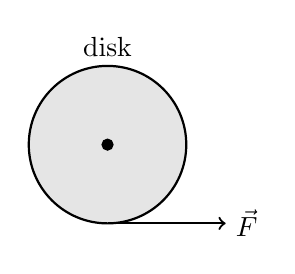
\begin{tikzpicture}
        %% Loop
        \node[anchor=south] at (0,1) {disk};
        \draw[thick,fill=white!90!black] (0,0) circle (1cm);
        \draw[fill] (0,0) circle (2pt);
        %% force
        \draw[thick,->] (0,-1) -- (1.5,-1) node[anchor=west] {$\vec{F}$};
    \end{tikzpicture}
    \hspace{\baselineskip}
    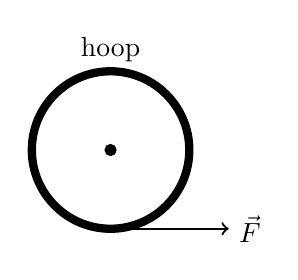
\begin{tikzpicture}
        %% Loop
        \node[anchor=south] at (0,1) {hoop};
        \draw[line width=3pt] (0,0) circle (1cm);
        \draw[fill] (0,0) circle (2pt);
        %% force
        \draw[thick,->] (0,-1) -- (1.5,-1) node[anchor=west] {$\vec{F}$};
    \end{tikzpicture}
    \vspace{\baselineskip}
    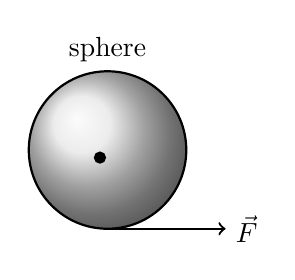
\begin{tikzpicture}
        %% Loop
        \node[anchor=south] at (0,1) {sphere};
        \draw[thick,shading=ball,ball color=white!90!black] (0,0) circle (1cm);
        \draw[fill] (0,0,0.25) circle (2pt);
        %% force
        \draw[thick,->] (0,-1) -- (1.5,-1) node[anchor=west] {$\vec{F}$};
    \end{tikzpicture}
    \end{center}
    Rank the objects according to their angular momenta after a given time $t$,
        least to greatest.
    \begin{multicols}{2}
    \begin{choices}
      \correctchoice{all tie}
        \wrongchoice{disk, hoop, sphere}
        \wrongchoice{hoop, disk, sphere}
        \wrongchoice{hoop, sphere, disk}
        \wrongchoice{hoop, disk, sphere}
    \end{choices}
    \end{multicols}
\end{question}
}

\element{halliday-mc}{
\begin{question}{halliday-ch11-q39}
    A single force acts on a particle $P$. 
    \begin{center}
    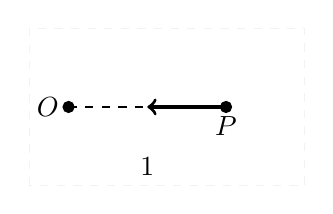
\begin{tikzpicture}
        \draw[dashed,white!95!black] (-1.5,-1) rectangle (2,1);
        \draw[fill] (-1,0) circle (2pt) node[anchor=east] {$O$};
        \draw[fill] (+1,0) circle (2pt) node[anchor=north] {$P$};
        \draw[dashed] (-1,0) -- (+1,0);
        \draw[very thick,->] (+1,0) -- (0,0);
        \node[anchor=south] at (0,-1) {1};
    \end{tikzpicture}
    \hspace{1em}
    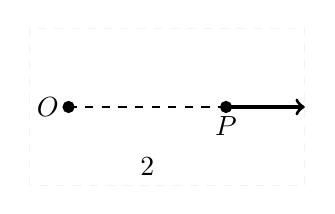
\begin{tikzpicture}
        \draw[dashed,white!95!black] (-1.5,-1) rectangle (2,1);
        \draw[fill] (-1,0) circle (2pt) node[anchor=east] {$O$};
        \draw[fill] (+1,0) circle (2pt) node[anchor=north] {$P$};
        \draw[dashed] (-1,0) -- (+1,0);
        \draw[very thick,->] (+1,0) -- (2,0);
        \node[anchor=south] at (0,-1) {2};
    \end{tikzpicture} \\
    \vspace{2em}
    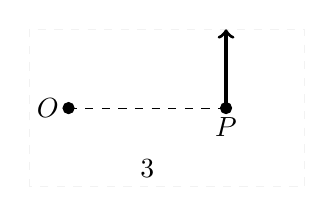
\begin{tikzpicture}
        \draw[dashed,white!95!black] (-1.5,-1) rectangle (2,1);
        \draw[fill] (-1,0) circle (2pt) node[anchor=east] {$O$};
        \draw[fill] (+1,0) circle (2pt) node[anchor=north] {$P$};
        \draw[dashed] (-1,0) -- (+1,0);
        \draw[very thick,->] (+1,0) -- (1,1);
        \node[anchor=south] at (0,-1) {3};
    \end{tikzpicture}
    \hspace{1em}
    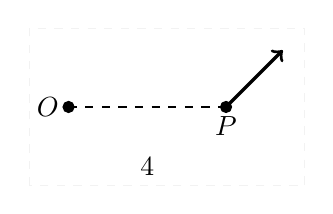
\begin{tikzpicture}
        \draw[dashed,white!95!black] (-1.5,-1) rectangle (2,1);
        \draw[fill] (-1,0) circle (2pt) node[anchor=east] {$O$};
        \draw[fill] (+1,0) circle (2pt) node[anchor=north] {$P$};
        \draw[dashed] (-1,0) -- (+1,0);
        \draw[very thick,->] (+1,0) -- (1.72,0.72);
        \node[anchor=south] at (0,-1) {4};
    \end{tikzpicture}
    \end{center}
    Rank each of the orientations of the force shown below according to the magnitude of the time rate of change of the particle's angular momentum about the point $O$,
        least to greatest.
    \begin{choices}
        \wrongchoice{1, 2, 3, 4}
        \wrongchoice{1 and 2 tie, then 3, 4}
      \correctchoice{1 and 2 tie, then 4, 3}
        \wrongchoice{1 and 2 tie, then 3 and 4 tie}
        \wrongchoice{All are the same}
    \end{choices}
\end{question}
}

\element{halliday-mc}{
\begin{question}{halliday-ch11-q40}
    A pulley with radius $R$ is free to rotate on a horizontal fixed axis through its center. 
    A string passes over the pulley. 
    Mass $m_1$ is attached to one end and mass $m_2$ is attached to the other.
    The portion of the string attached to $m_1$ has tension $T_1$ and the portion attached to $m_2$ has tension $T_2$.
    The magnitude of the total external torque,
        about the pulley center, acting on the masses and pulley, considered as a system, is given by:
    \begin{choices}
      \correctchoice{$\left|m_1 - m_2\right| gR$}
        \wrongchoice{$\left(m_1 + m_2\right) gR$}
        \wrongchoice{$\left|m_1 - m_2\right| gR + \left(T_1 + T_2\right) R$}
        \wrongchoice{$\left(m_1 + m_2\right) gR + \left(T_1 - T_2\right) R$}
        \wrongchoice{$\left|m_1 - m_2\right| gR + \left(T_2 - T_1\right) R$}
    \end{choices}
\end{question}
}

\element{halliday-mc}{
\begin{question}{halliday-ch11-q41}
    An ice skater with rotational inertia $I_0$ is spinning with angular speed $\omega_0$. 
    She pulls her arms in,
        thereby increasing her angular speed to $4\omega_0$. 
    Her rotational inertia is then:
    \begin{multicols}{3}
    \begin{choices}
        \wrongchoice{$I_0$}
        \wrongchoice{$\dfrac{I_0}{2}$}
        \wrongchoice{$2I_0$}
      \correctchoice{$\dfrac{I_0}{4}$}
        \wrongchoice{$4I_0$}
    \end{choices}
    \end{multicols}
\end{question}
}

\element{halliday-mc}{
\begin{question}{halliday-ch11-q42}
    A man, with his arms at his sides,
        is spinning on a light frictionless turntable. 
    When he extends his arms:
    \begin{choices}
        \wrongchoice{his angular velocity increases}
        \wrongchoice{his angular velocity remains the same}
        \wrongchoice{his rotational inertia decreases}
        \wrongchoice{his rotational kinetic energy increases}
      \correctchoice{his angular momentum remains the same}
    \end{choices}
\end{question}
}

\element{halliday-mc}{
\begin{question}{halliday-ch11-q43}
    A man, holding a weight in each hand,
        stands at the center of a horizontal frictionless rotating turntable. 
    The effect of the weights is to double the rotational inertia of the system. 
    As he is rotating, the man opens his hands and drops the two weights. 
    They fall outside the turntable.
    Then:
    \begin{choices}
        \wrongchoice{his angular velocity doubles}
      \correctchoice{his angular velocity remains about the same}
        \wrongchoice{his angular velocity is halved}
        \wrongchoice{the direction of his angular momentum vector changes}
        \wrongchoice{his rotational kinetic energy increases}
    \end{choices}
\end{question}
}

\element{halliday-mc}{
\begin{question}{halliday-ch11-q44}
    A uniform sphere of radius $R$ rotates about a diameter with an angular momentum of magnitude $L$. 
    Under the action of internal forces the sphere collapses to a uniform sphere of radius $R/2$.
    The magnitude of its new angular momentum is:
    \begin{multicols}{3}
    \begin{choices}
        \wrongchoice{$\dfrac{L}{4}$}
        \wrongchoice{$\dfrac{L}{2}$}
      \correctchoice{$L$}
        \wrongchoice{$2L$}
        \wrongchoice{$4L$}
    \end{choices}
    \end{multicols}
\end{question}
}

\element{halliday-mc}{
\begin{question}{halliday-ch11-q45}
    When a man on a frictionless rotating stool extends his arms horizontally,
        his rotational kinetic energy:
    \begin{choices}
        \wrongchoice{must increase}
      \correctchoice{must decrease}
        \wrongchoice{must remain the same}
        \wrongchoice{may increase or decrease depending on his initial angular velocity}
        \wrongchoice{may increase or decrease depending on his angular acceleration}
    \end{choices}
\end{question}
}

\element{halliday-mc}{
\begin{question}{halliday-ch11-q46}
    When a woman on a frictionless rotating turntable extends her arms out horizontally,
        her angular momentum:
    \begin{choices}
        \wrongchoice{must increase}
        \wrongchoice{must decrease}
      \correctchoice{must remain the same}
        \wrongchoice{may increase or decrease depending on her initial angular velocity}
        \wrongchoice{tilts away from the vertical}
    \end{choices}
\end{question}
}

\element{halliday-mc}{
\begin{question}{halliday-ch11-q47}
    Two disks are mounted on low-friction bearings on a common shaft. 
    The first disc has rotational inertia $I$ and is spinning with angular velocity $\omega$. 
    The second disc has rotational inertia $2I$ and is spinning in the same direction as the first disc with angular velocity $2\omega$ as shown. 
    \begin{center}
    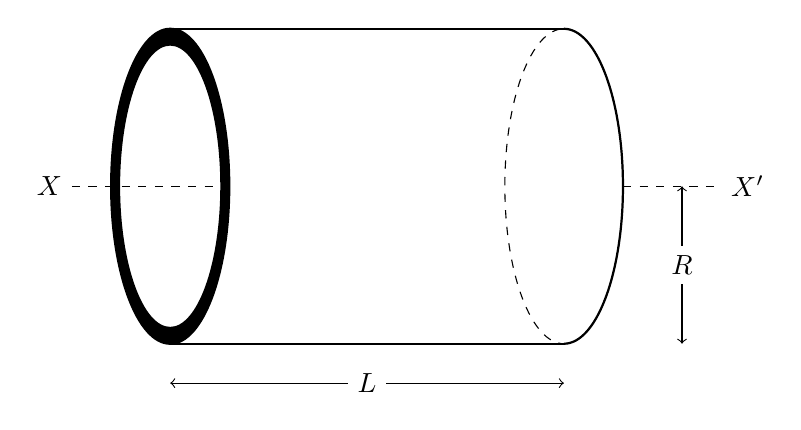
\begin{tikzpicture}
        %% NOTE: tikz 3D
        %% bar
        %% Barrel
        \draw[thick,fill] (0,0) circle (0.75cm and 2cm);
        \draw[thick,fill=white] (0,0) circle (0.65cm and 1.8cm);
        \draw[dashed] (5,0) circle (0.75cm and 2cm);
        \draw[thick] (5,-2) arc (-90:90:0.75cm and 2cm);
        \draw[thick] (0,2) -- (5,2);
        \draw[thick] (0,-2) -- (5,-2);
        %% Labels
        \draw[dashed] (-1.25,0) -- (0.75,0) node[pos=0.0,anchor=east] {$X$};
        \draw[dashed] (5.75,0) -- (7.0,0) node[pos=1.0,anchor=west] {$X^{\prime}$};
        \draw[<->] (6.5,0) -- (6.5,-2) node[pos=0.5,anchor=center,fill=white] {$R$};
        \draw[<->] (0,-2.5) -- (5,-2.5) node[pos=0.5,anchor=center,fill=white] {$L$};
    \end{tikzpicture}
    \end{center}
    The two disks are slowly forced toward each other along the shaft until they couple and have a final common angular velocity of:
    \begin{multicols}{3}
    \begin{choices}
      \correctchoice{$\dfrac{5\omega}{3}$}
        \wrongchoice{$\omega\sqrt{3}$}
        \wrongchoice{$\omega\sqrt{\dfrac{7}{3}}$}
        \wrongchoice{$\omega$}
        \wrongchoice{$3\omega$}
    \end{choices}
    \end{multicols}
\end{question}
}

\element{halliday-mc}{
\begin{question}{halliday-ch11-q48}
    A wheel with rotational inertia $I$, 
        mounted on a vertical shaft with negligible rotational inertia,
        is rotating with angular speed $\omega_0$. 
    A nonrotating wheel with rotational inertia $2I$ is suddenly dropped onto the same shaft as shown. 
    \begin{center}
    \begin{tikzpicture}
        %% NOTE: tikz 3D
    \end{tikzpicture}
    \end{center}
    The resultant combination of the two wheels and shaft will rotate at:
    \begin{multicols}{3}
    \begin{choices}
        \wrongchoice{$\dfrac{\omega_0}{2}$}
        \wrongchoice{$2\omega_0$}
      \correctchoice{$\dfrac{\omega_0}{3}$}
        \wrongchoice{$3\omega_0$}
        \wrongchoice{$\dfrac{\omega_0}{4}$}
    \end{choices}
    \end{multicols}
\end{question}
}

\element{halliday-mc}{
\begin{question}{halliday-ch11-q49}
    A phonograph record is dropped onto a freely spinning turntable. 
    Then:
    \begin{choices}
        \wrongchoice{neither angular momentum nor mechanical energy is conserved because of the frictional forces between record and turntable}
        \wrongchoice{the frictional force between record and turntable increases the total angular momentum}
        \wrongchoice{the frictional force between record and turntable decreases the total angular momentum}
      \correctchoice{the total angular momentum remains constant}
        \wrongchoice{the sum of the angular momentum and rotational kinetic energy remains constant}
    \end{choices}
\end{question}
}

\element{halliday-mc}{
\begin{question}{halliday-ch11-q50}
    A playground merry-go-round has a radius R and a rotational inertia $I$. 
    When the merry-go-round is at rest,
        a child with mass m runs with speed $v$ along a line tangent to the rim and jumps on. 
    The angular velocity of the merry-go-round is then:
    \begin{multicols}{3}
    \begin{choices}
        \wrongchoice{$\dfrac{mv}{I}$}
        \wrongchoice{$\dfrac{v}{R}$}
        \wrongchoice{$\dfrac{mRv}{I}$}
        \wrongchoice{$\dfrac{2mRv}{I}$}
      \correctchoice{$\dfrac{mRv}{mR^2 + I}$}
    \end{choices}
    \end{multicols}
\end{question}
}

\element{halliday-mc}{
\begin{question}{halliday-ch11-q51}
    A playground merry-go-round has a radius of \SI{3.0}{\meter} and a rotational inertia of \SI{600}{\kilo\gram\meter\squared}.
    It is initially spinning at \SI{0.80}{\radian\per\second} when a \SI{20}{\kilo\gram} child crawls from the center to the rim. 
    When the child reaches the rim the angular velocity of the merry-go-round is:
    \begin{multicols}{3}
    \begin{choices}
      \correctchoice{\SI{0.62}{\radian\per\second}}
        \wrongchoice{\SI{0.73}{\radian\per\second}}
        \wrongchoice{\SI{0.80}{\radian\per\second}}
        \wrongchoice{\SI{0.89}{\radian\per\second}}
        \wrongchoice{\SI{1.1}{\radian\per\second}}
    \end{choices}
    \end{multicols}
\end{question}
}

\element{halliday-mc}{
\begin{question}{halliday-ch11-q52}
    Two pendulum bobs of unequal mass are suspended from the same fixed point by strings of equal length.
    The lighter bob is drawn aside and then released so that it collides with the other bob on reaching the vertical position. 
    The collision is elastic. 
    What quantities are conserved in the collision?
    \begin{choices}
      \correctchoice{Both kinetic energy and angular momentum of the system}
        \wrongchoice{Only kinetic energy}
        \wrongchoice{Only angular momentum}
        \wrongchoice{Angular speed of lighter bob}
        \wrongchoice{None of the provided}
    \end{choices}
\end{question}
}

\element{halliday-mc}{
\begin{question}{halliday-ch11-q53}
    A particle, held by a string whose other end is attached to a fixed point $C$,
        moves in a circle on a horizontal frictionless surface. 
    If the string is cut,
        the angular momentum of the particle about the point $C$:
    \begin{choices}
        \wrongchoice{increases}
        \wrongchoice{decreases}
      \correctchoice{does not change}
        \wrongchoice{changes direction but not magnitude}
        \wrongchoice{none of these}
    \end{choices}
\end{question}
}

\element{halliday-mc}{
\begin{question}{halliday-ch11-q54}
    A block with mass $M$, on the end of a string,
        moves in a circle on a horizontal frictionless table as shown. 
    \begin{center}
    \begin{tikzpicture}
        %% NOTE: tikz 3D
    \end{tikzpicture}
    \end{center}
    As the string is slowly pulled through a small hole in the table:
    \begin{choices}
      \correctchoice{the angular momentum of the block remains constant}
        \wrongchoice{the angular momentum of the block decreases}
        \wrongchoice{the kinetic energy of the block remains constant}
        \wrongchoice{the kinetic energy of the block decreases}
        \wrongchoice{none of the above}
    \end{choices}
\end{question}
}


\endinput


